\subsection{System Test}
%The sokoban solver was implemented as an A* algorithm in C++ with focus on memory consumption and processing time.
%In order to test quantify the final program then this is tested in regards of these factors.

%The program was written for single core processing only and executed on a Intel Core i7-3610QM running at 2.3GHz with a total of 8GB RAM running Ubuntu.

The program was first tested on the handed out test map from the competition of year 2014.
This was used to see if the solution found was as short as path supplied and to consider the memory consumption and processing time of the program.

The path found by the program was, like the solution provided, 124 steps indicating that the solver is capable of returning the right result.
The memory used by the program is seen in figure \ref{fig:memoryconsumption2014}.


As seen on figure \ref{fig:memoryconsumption2014}, then the memory consumption is just below 30MB.
Where the main memory consumption is from the openlist (red), the strings used for hashing (yellow), and the closed list (green).

The solver was furthermore tested on a set of different microban maps to see if the program works and this was confirmed.
Theoretically the solver can solve any map, as long as it has enough time and memory to do so.


\begin{figure}[H]
\centering
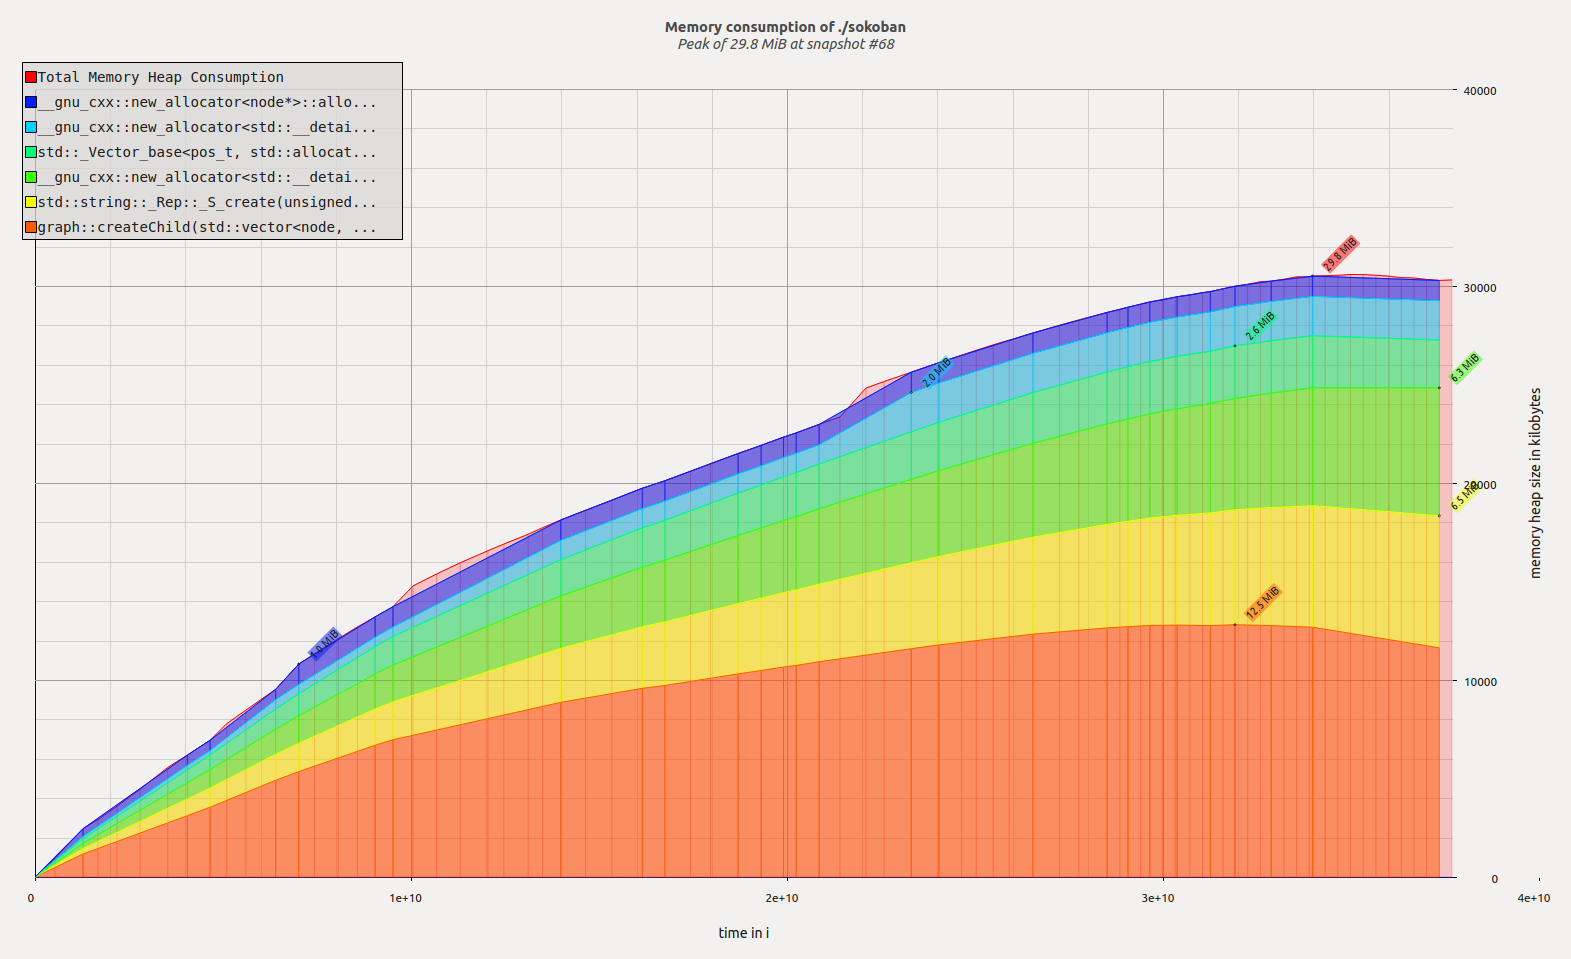
\includegraphics[width = 0.8 \linewidth]{graphics/memoryconsumption.png}
\caption{Memory consumption of the program when computing the solution for the competition of year 2014.}
\label{fig:memoryconsumption2014}
\end{figure}

In its current version, the map size is however limited to to maps with a total map size less or equal to 255 squares.
This is due to the implementation of the closed list and the choice of hashing value.
%It can however be increased at a cost of more memory used per node in the table.




